\documentclass[article, 11pt, oneside]{memoir}
\usepackage{Sweave}
\usepackage[OT1]{fontenc}
\usepackage[utf8]{inputenc}
\begin{document}

% \VignetteIndexEntry{SDAusingsurvey}

\title{Reproduction of Analyses in Lohr (1999)\\ 
       using the \texttt{survey} package}
\author{Tobias Verbeke}
\date{2009-09-15}
\maketitle

\begin{Schunk}
\begin{Sinput}
> library(SDA)
> library(survey)
\end{Sinput}
\end{Schunk}

\chapter{Chapter 3: Ratio and Regression Estimation}

\begin{Schunk}
\begin{Sinput}
> pf <- data.frame(photo = c(10, 12, 7, 13, 13, 6, 17, 16, 15, 
+     10, 14, 12, 10, 5, 12, 10, 10, 9, 6, 11, 7, 9, 11, 10, 10), 
+     field = c(15, 14, 9, 14, 8, 5, 18, 15, 13, 15, 11, 15, 12, 
+         8, 13, 9, 11, 12, 9, 12, 13, 11, 10, 9, 8))
\end{Sinput}
\end{Schunk}

\begin{Schunk}
\begin{Sinput}
> df <- data.frame(tree = 1:10, x = c(1, 0, 8, 2, 76, 60, 25, 2, 
+     1, 31), y = c(0, 0, 1, 2, 10, 15, 3, 2, 1, 27))
> names(df) <- c("tree", "x", "y")
\end{Sinput}
\end{Schunk}


\chapter{Chapter 5}

\begin{Schunk}
\begin{Sinput}
> txt <- "person_num cluster gpa\n  1 1 3.08\n  2 1 2.60\n  3 1 3.44\n  4 1 3.04\n  1 2 2.36\n  2 2 3.04\n  3 2 3.28\n  4 2 2.68\n  1 3 2.00\n  2 3 2.56\n  3 3 2.52\n  4 3 1.88\n  1 4 3.00\n  2 4 2.88\n  3 4 3.44\n  4 4 3.64\n  1 5 2.68\n  2 5 1.92\n  3 5 3.28\n  4 5 3.20"
> txtConn <- textConnection(txt)
> GPA <- read.table(txtConn, header = TRUE)
> GPA$pwt <- 100/5
> clusterDesign <- svydesign(ids = ~cluster, weights = ~pwt, data = GPA)
> svytotal(~gpa, design = clusterDesign)
\end{Sinput}
\begin{Soutput}
     total     SE
gpa 1130.4 67.167
\end{Soutput}
\end{Schunk}

\chapter{Chapter 6: Sampling with Unequal Probabilities}

% cf. 
% http://statistics.ats.ucla.edu/stat/stata/examples/lohr/lohrstata6.htm
%

\begin{Schunk}
\begin{Sinput}
> data(statepop)
> statepop$psi <- statepop$popn/255077536
\end{Sinput}
\end{Schunk}

\begin{Schunk}
\begin{Sinput}
> plot(phys ~ psi, data = statepop, xlab = expression(paste(Psi[i], 
+     " for County")), ylab = "Physicians in County (in thousands)")
\end{Sinput}
\end{Schunk}
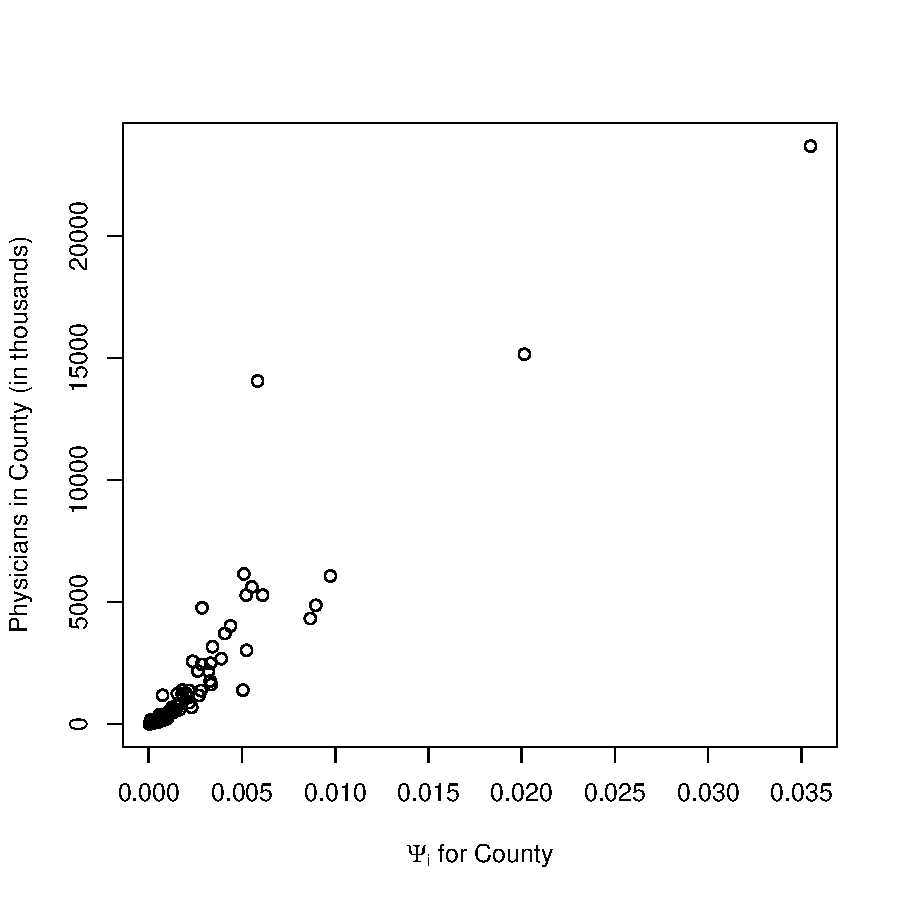
\includegraphics{SDA_using_survey-006}

% TODO aanvullen met rest van gegevens op pagina

\chapter{Chapter 7: Complex Surveys}

\section{Estimating a Distribution Function}

\begin{Schunk}
\begin{Sinput}
> data(htpop)
> popecdf <- ecdf(htpop$height)
> plot(popecdf, do.points = FALSE, ylab = "F(y)", xlab = "Height Value, y")
\end{Sinput}
\end{Schunk}
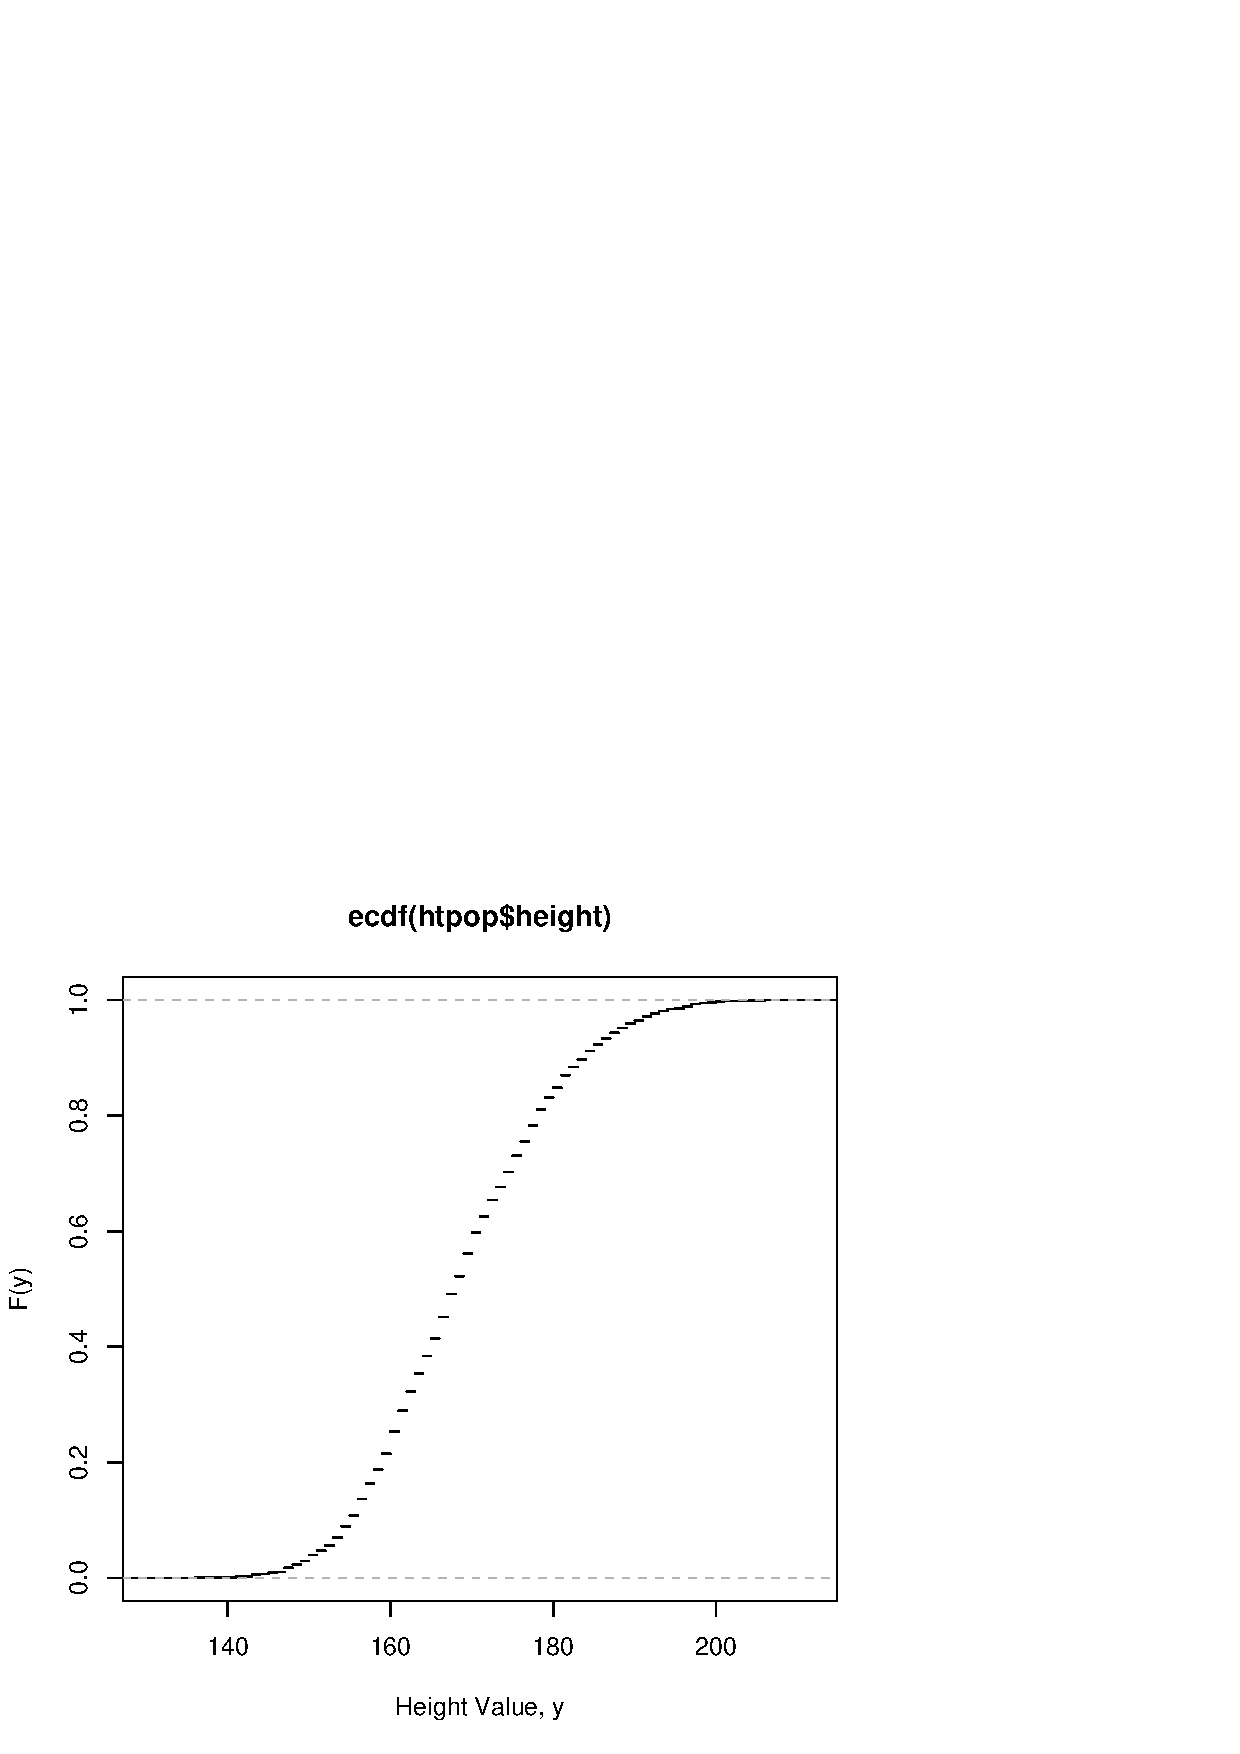
\includegraphics{SDA_using_survey-007}

\begin{Schunk}
\begin{Sinput}
> minht <- min(htpop$height)
> breaks <- c(minht - 1, seq(from = minht, to = max(htpop$height), 
+     by = 1))
> hist(htpop$height, ylab = "f(y)", breaks = breaks, xlab = "Height Value, y", 
+     freq = FALSE)
\end{Sinput}
\end{Schunk}
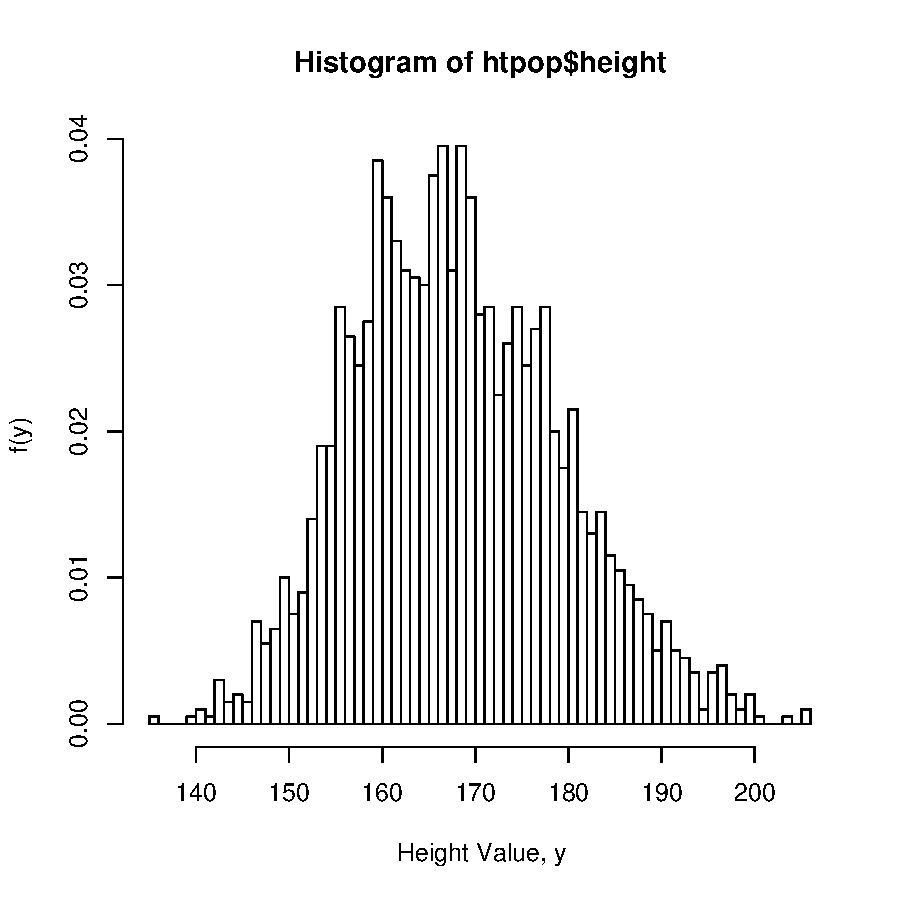
\includegraphics{SDA_using_survey-008}

\begin{Schunk}
\begin{Sinput}
> data(htsrs)
> hist(htsrs$height, ylab = "Relative Frequency", xlab = "Height (cm)", 
+     freq = FALSE)
\end{Sinput}
\end{Schunk}
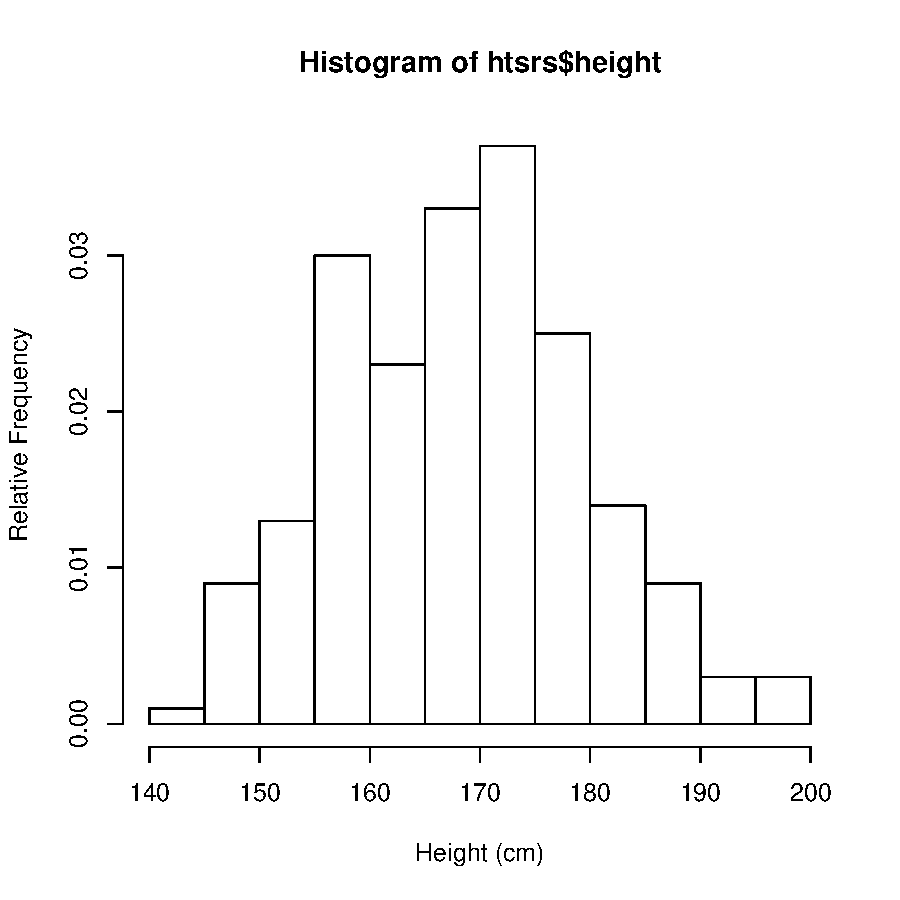
\includegraphics{SDA_using_survey-009}

% TODO Figure 7.3 can be improved (change number of breaks) 

\begin{Schunk}
\begin{Sinput}
> data(htstrat)
> hist(htstrat$height, ylab = "Relative Frequency", xlab = "Height (cm)", 
+     freq = FALSE)
\end{Sinput}
\end{Schunk}
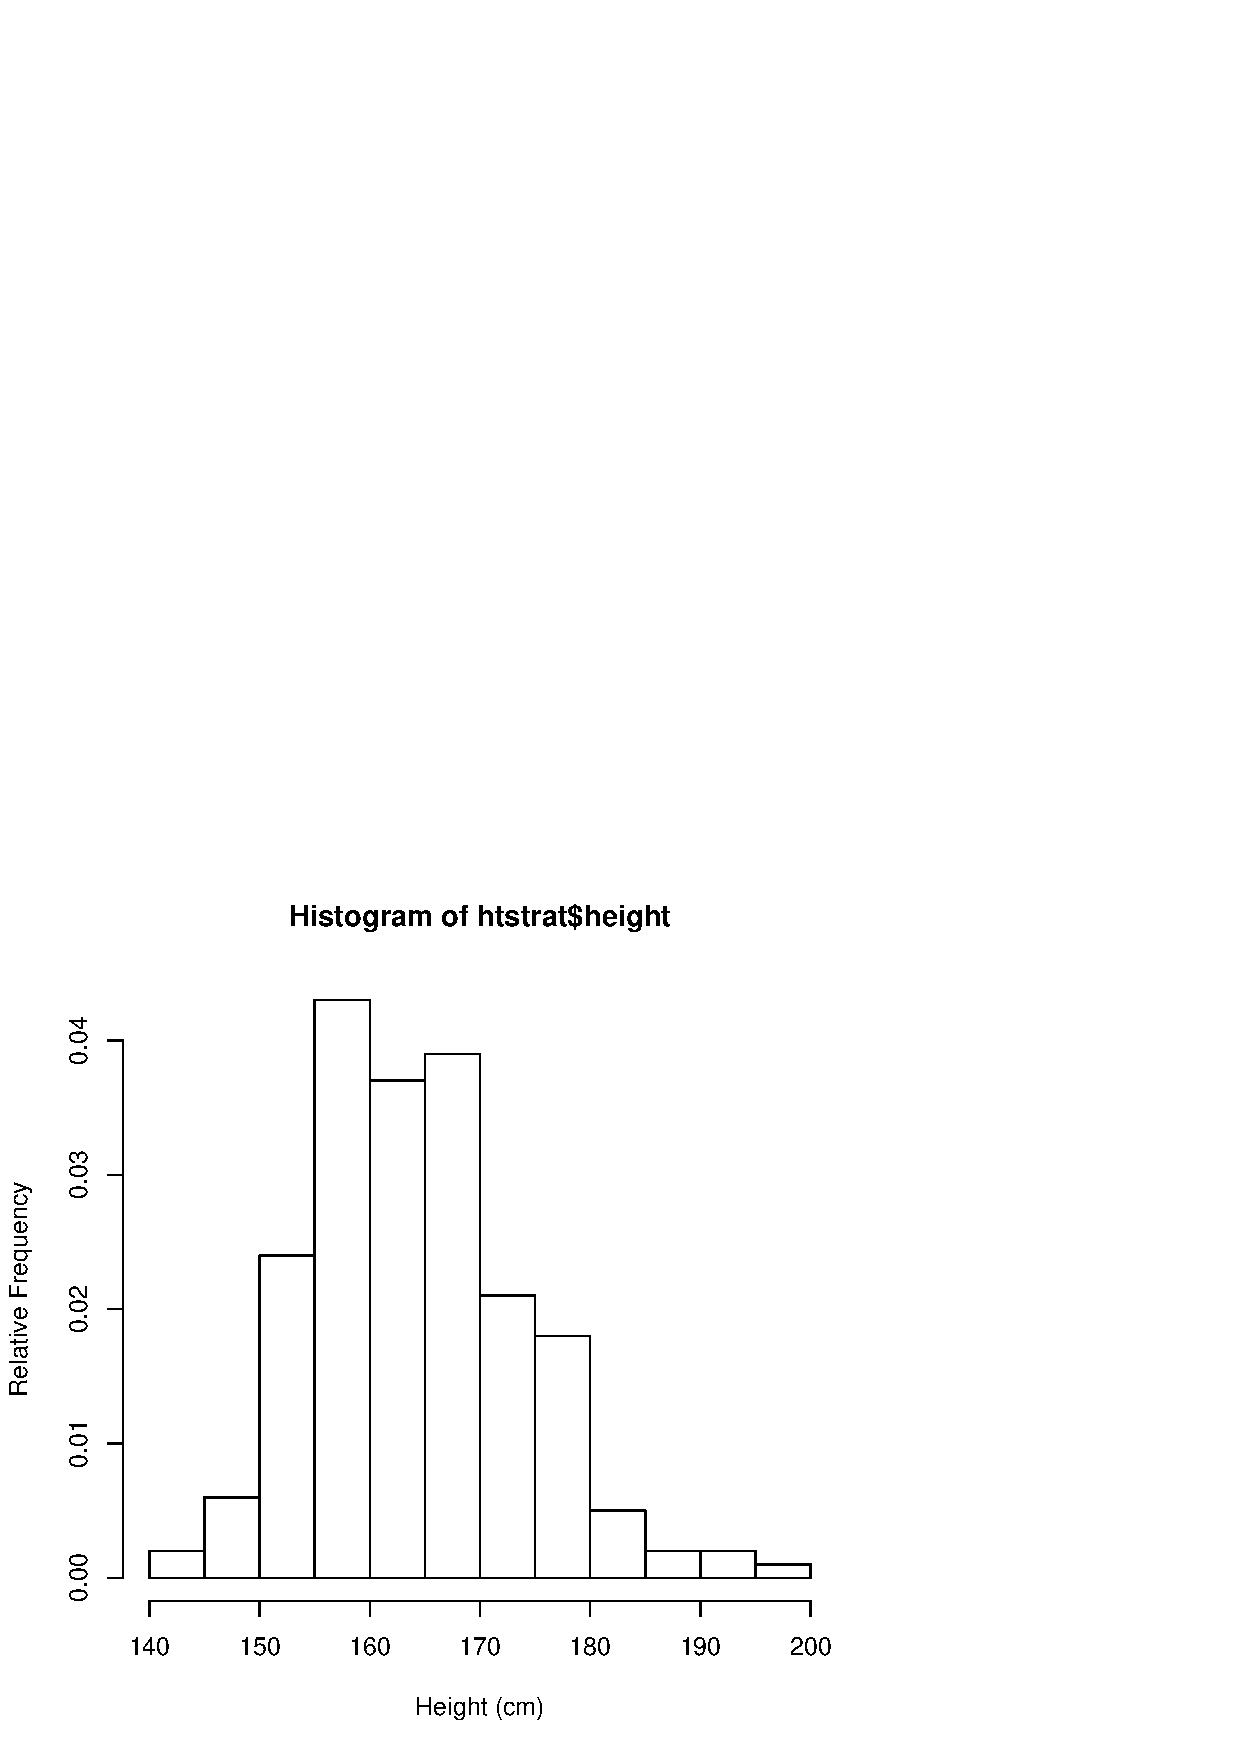
\includegraphics{SDA_using_survey-010}

\begin{Schunk}
\begin{Sinput}
> minht <- min(htstrat$height)
> breaks <- c(minht - 1, seq(from = minht, to = max(htstrat$height), 
+     by = 1))
> hist(htstrat$height, ylab = expression(hat(f)(y)), breaks = breaks, 
+     xlab = "Height Value, y", freq = FALSE)
\end{Sinput}
\end{Schunk}
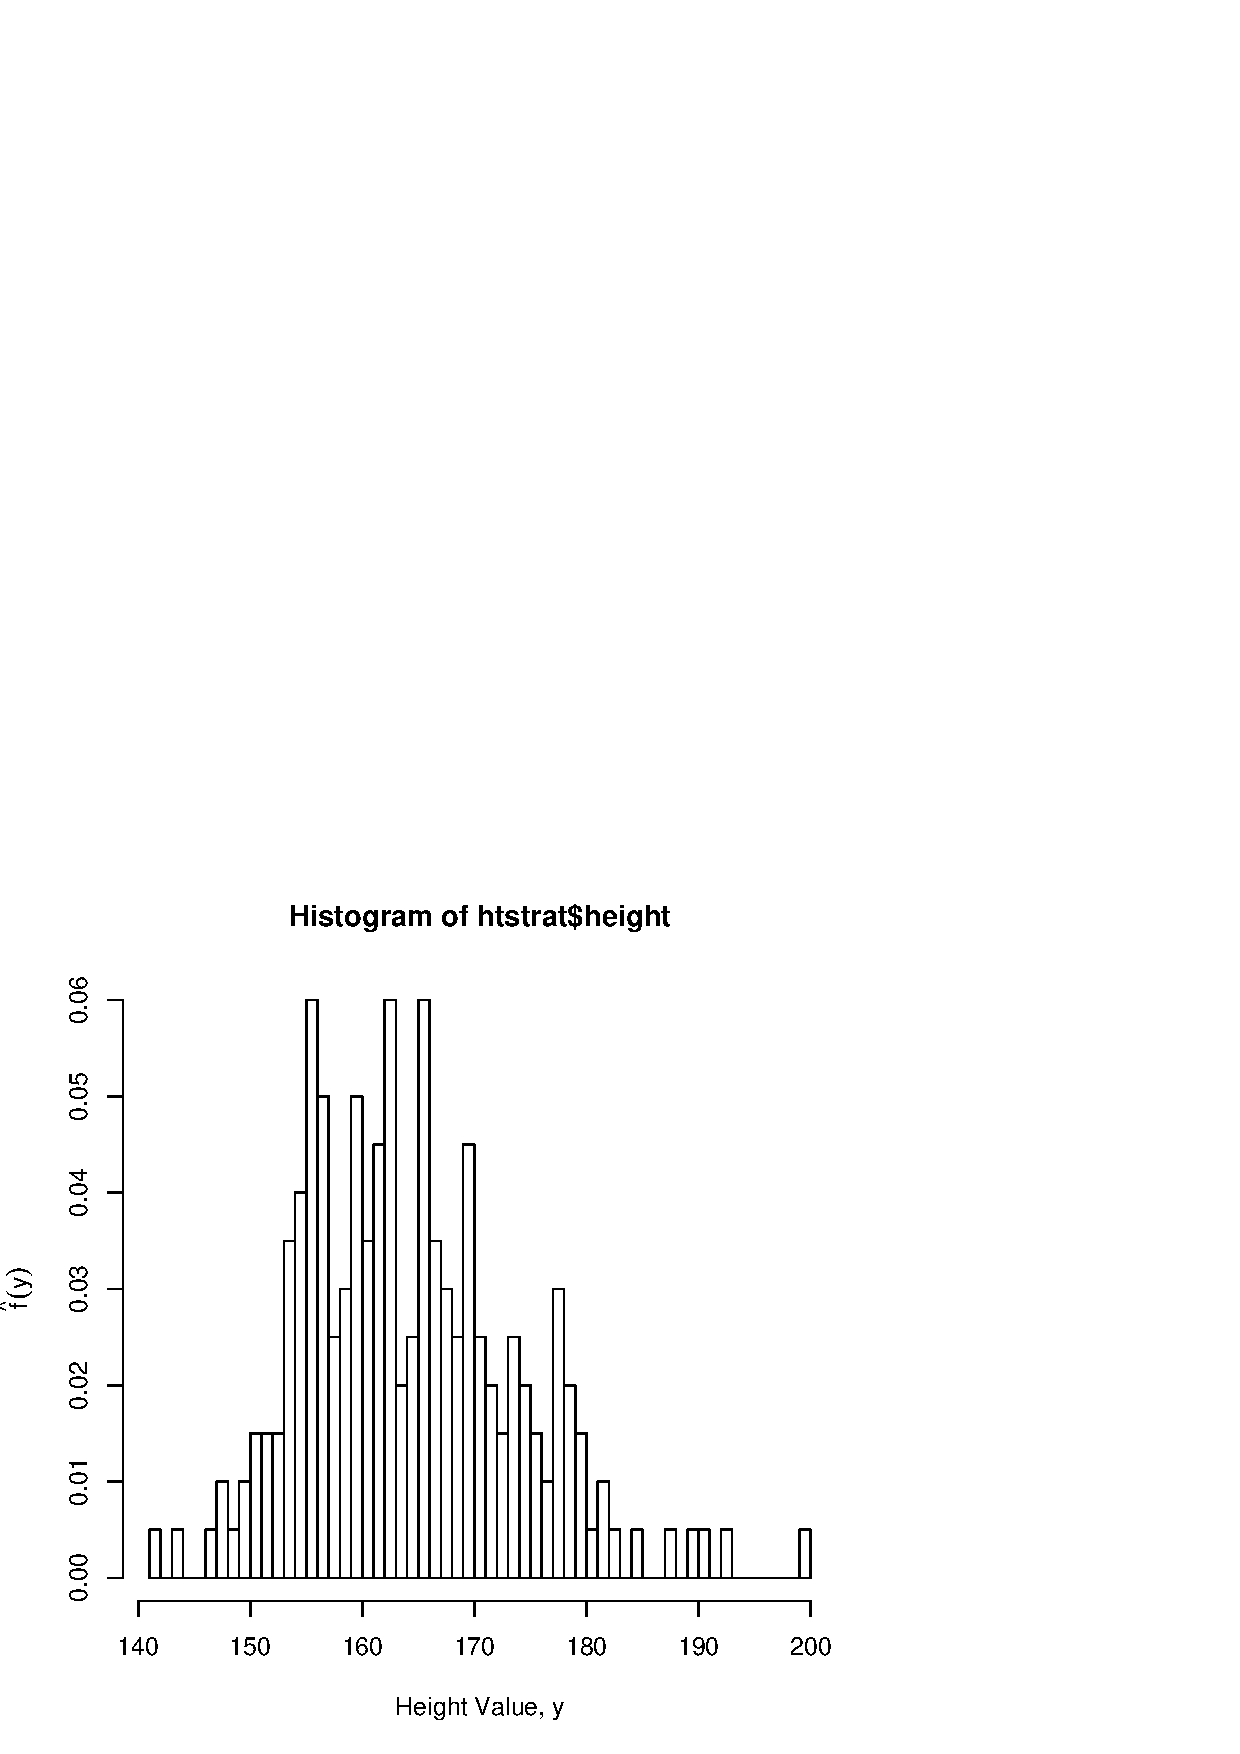
\includegraphics{SDA_using_survey-011}

\begin{Schunk}
\begin{Sinput}
> stratecdf <- ecdf(htstrat$height)
> plot(stratecdf, do.points = FALSE, ylab = expression(hat(F)(y)), 
+     xlab = "Height Value, y")
\end{Sinput}
\end{Schunk}
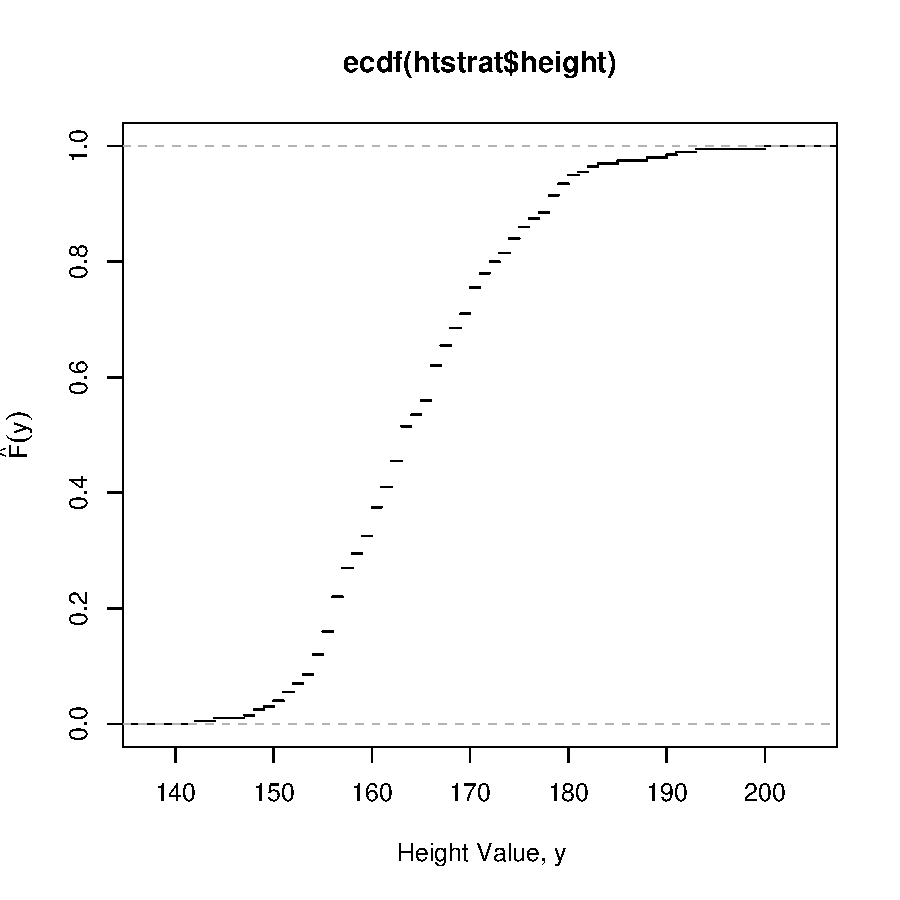
\includegraphics{SDA_using_survey-012}

\section{Plotting Data from a Complex Survey}

\begin{Schunk}
\begin{Sinput}
> data(syc)
> hist(syc$age, freq = FALSE, xlab = "Age")
\end{Sinput}
\end{Schunk}
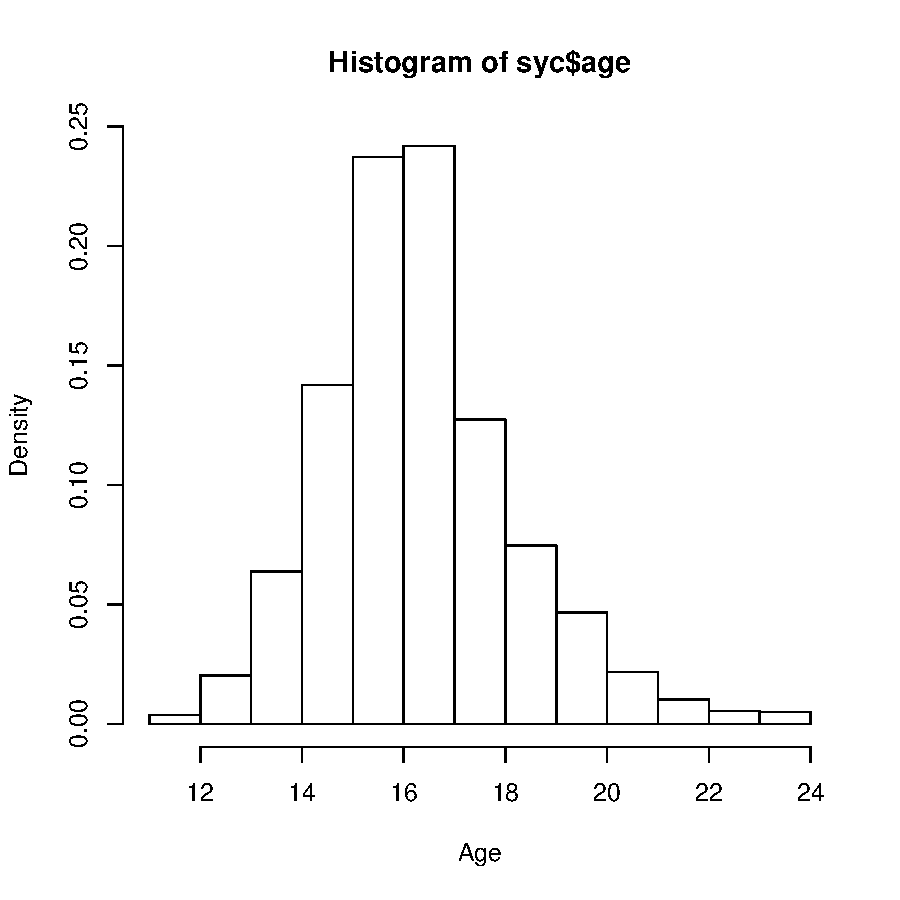
\includegraphics{SDA_using_survey-013}

% TODO add Figure 7.7 (?)

Note that in its current implementation, \texttt{svyboxplot} will
only plot minimum and maximum as outliers if they are situated 
outside the whiskers. Other outliers are not plotted 
(see \texttt{?svyboxplot}). This explains the minor difference with
Figure 7.8 on p. 237 of Lohr (1999).

\begin{Schunk}
\begin{Sinput}
> sycdesign <- svydesign(ids = ~psu, strata = ~stratum, data = syc, 
+     weights = ~finalwt)
> oo <- options(survey.lonely.psu = "certainty")
> svyboxplot(age ~ factor(stratum), design = sycdesign)
> options(oo)
\end{Sinput}
\end{Schunk}
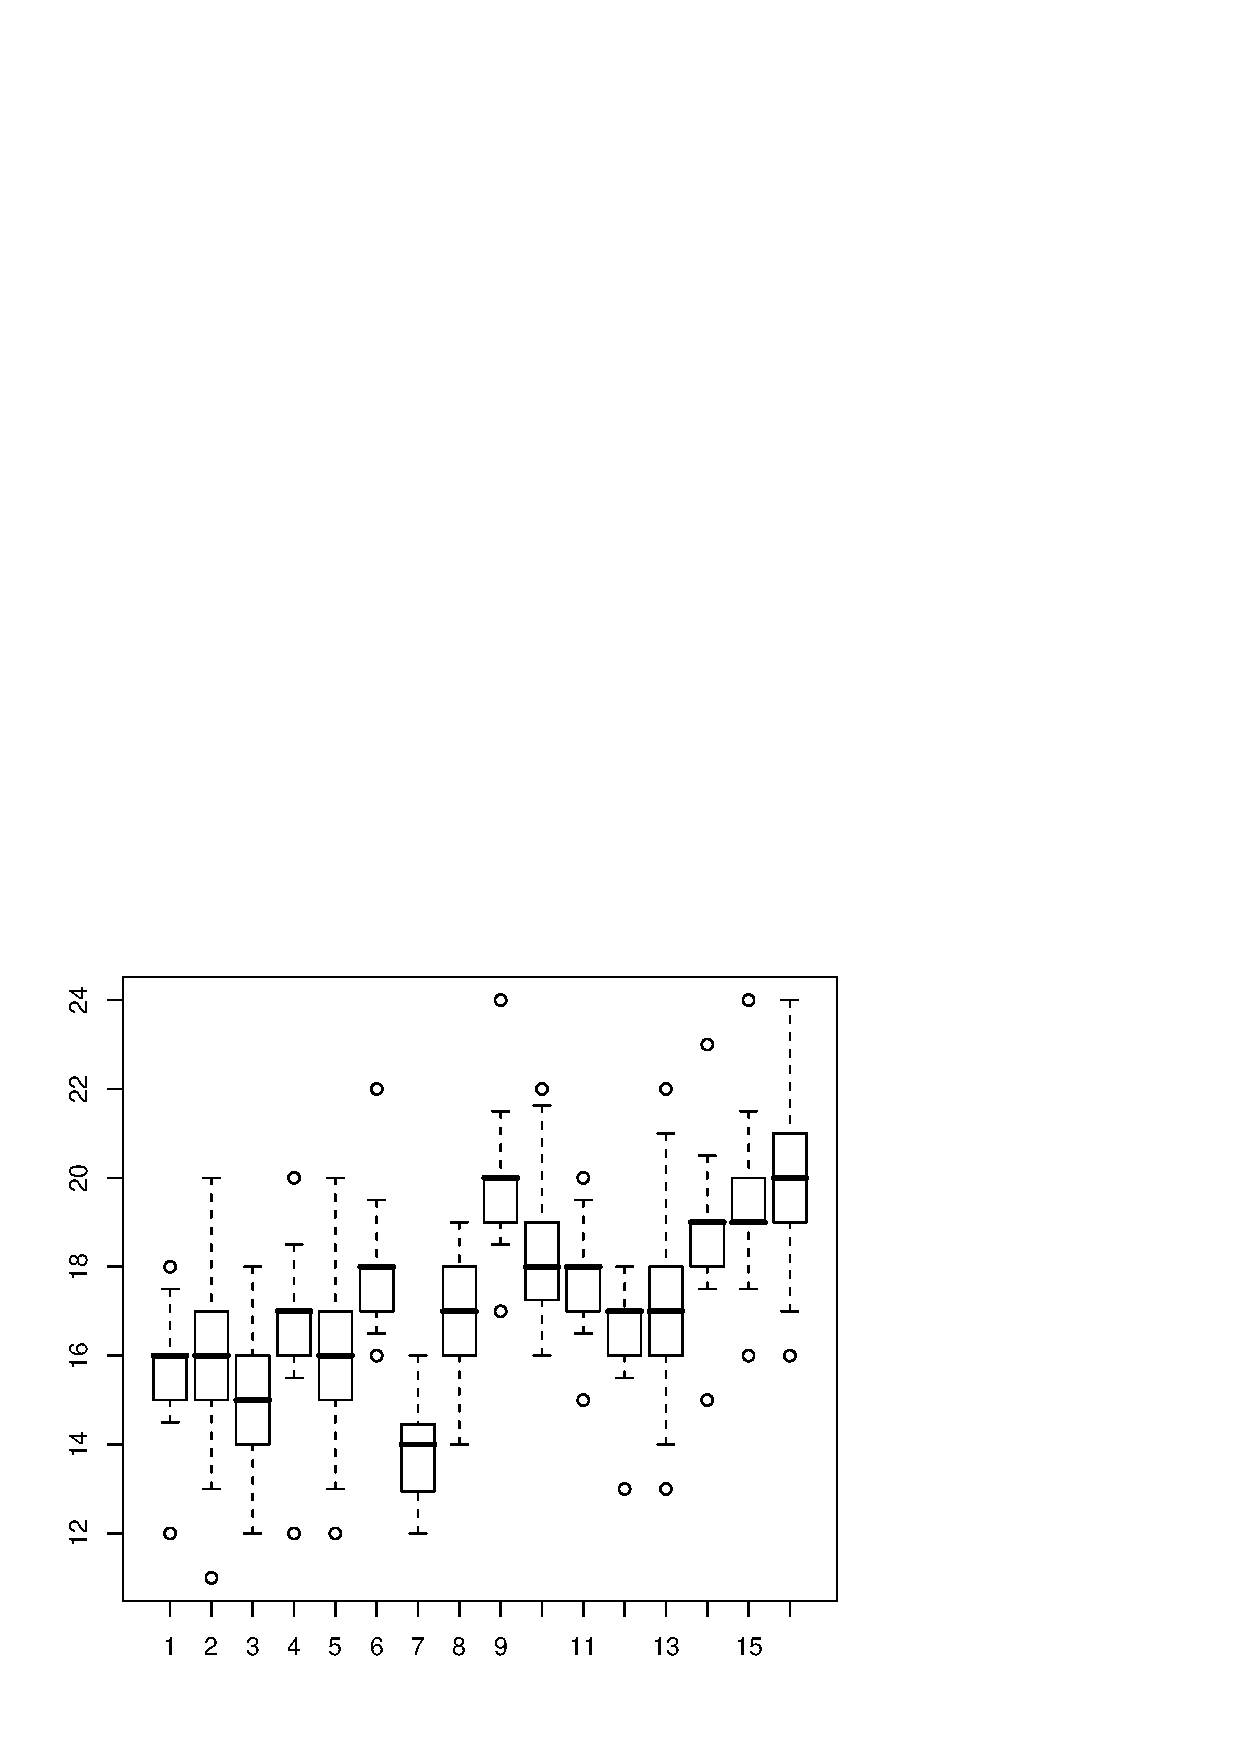
\includegraphics{SDA_using_survey-014}

This kind of plot is particularly easy to formulate
in the grammar of graphics, i.e. using the \texttt{ggplot2}
package~:

\begin{Schunk}
\begin{Sinput}
> p <- ggplot(syc, aes(x = factor(stratum), y = factor(age)))
> g <- p + stat_sum(aes(group = 1, weight = finalwt, size = ..sum..))
> print(g)
\end{Sinput}
\end{Schunk}
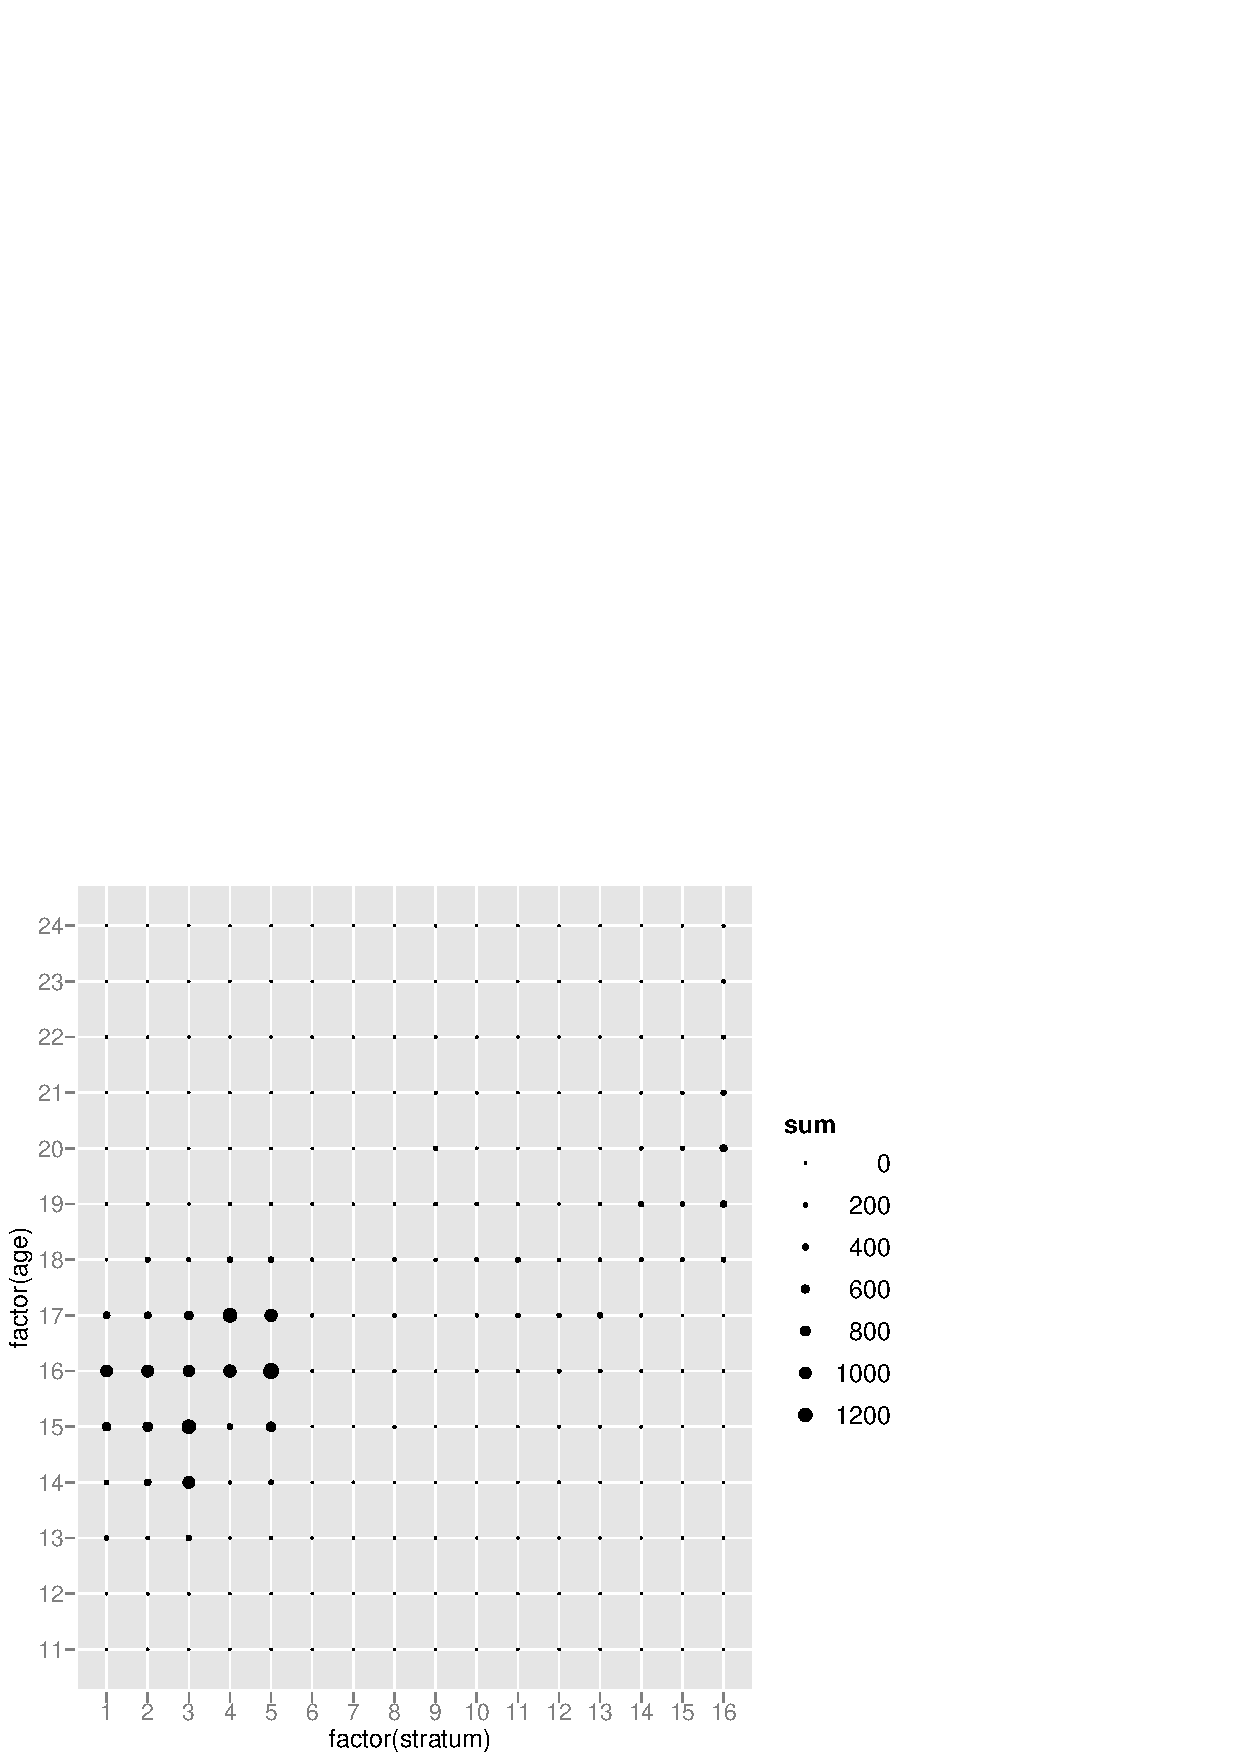
\includegraphics{SDA_using_survey-015}

% TODO: check that it is really the sum of finalwt that is displayed     
     
Note that in its current implementation, \texttt{svyboxplot} will
only plot minimum and maximum as outliers if they are situated 
outside the whiskers. Other outliers are not plotted 
(see \texttt{?svyboxplot}). This explains the minor difference with
Figure 7.10 on p. 238 of Lohr (1999).
 
     
\begin{Schunk}
\begin{Sinput}
> oo <- options(survey.lonely.psu = "certainty")
> sycstrat5 <- subset(sycdesign, stratum == 5)
> svyboxplot(age ~ factor(psu), design = sycstrat5)
> options(oo)
\end{Sinput}
\end{Schunk}
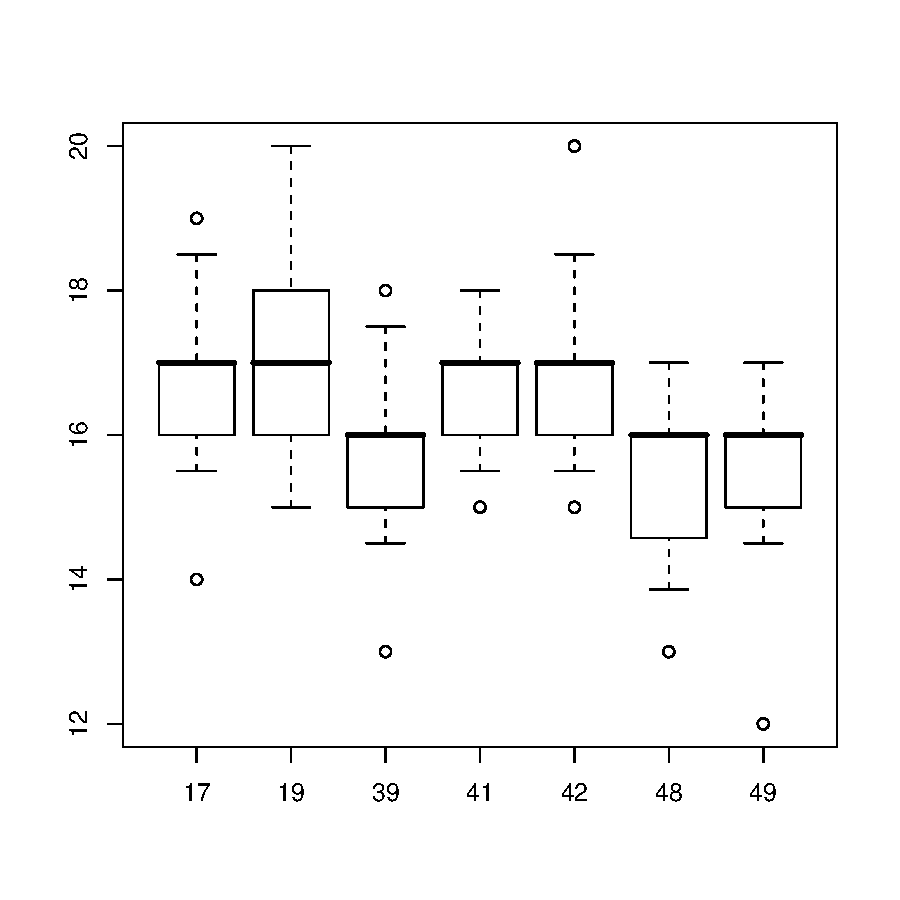
\includegraphics{SDA_using_survey-016}

\begin{Schunk}
\begin{Sinput}
> sycstrat5df <- subset(syc, stratum == 5)
> p <- ggplot(sycstrat5df, aes(x = factor(psu), y = factor(age)))
> g <- p + stat_sum(aes(group = 1, weight = finalwt, size = ..sum..))
> print(g)
\end{Sinput}
\end{Schunk}
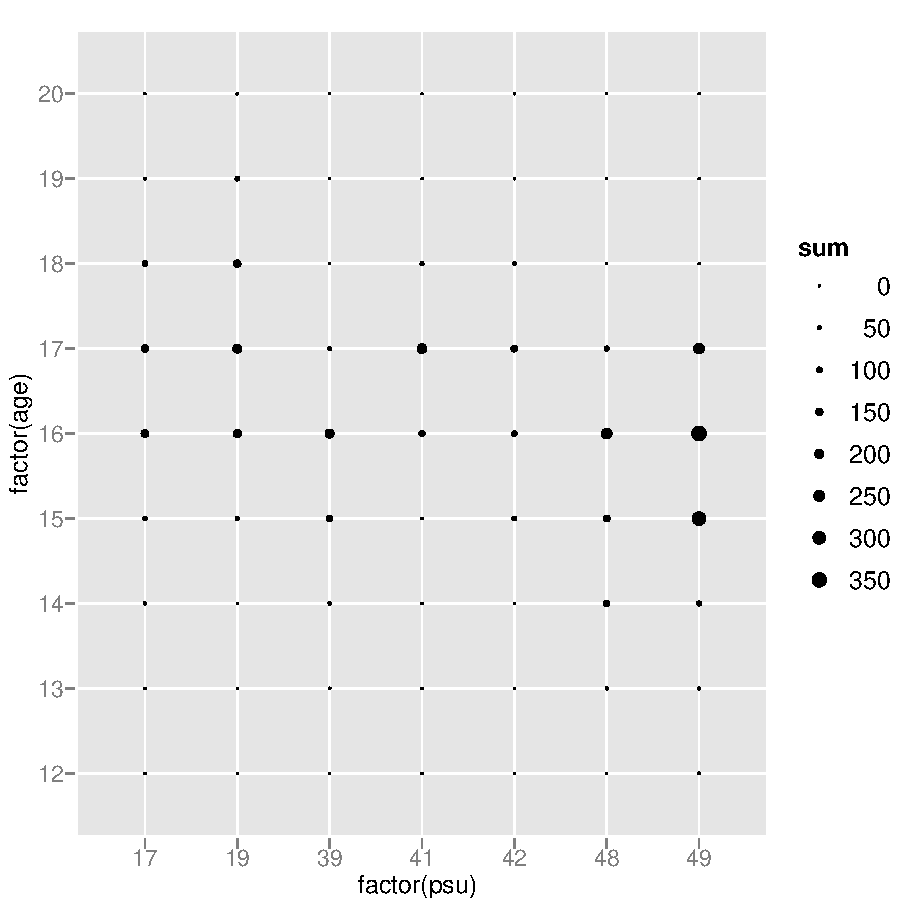
\includegraphics{SDA_using_survey-017}



\chapter{Chapter 10: Categorical Data Analysis in Complex Surveys}

\section{Chi-Square Tests with Multinomial Sampling}

\begin{Schunk}
\begin{Sinput}
> hh <- rbind(c(119, 188), c(88, 105))
> rownames(hh) <- c("cableYes", "cableNo")
> colnames(hh) <- c("computerYes", "computerNo")
> addmargins(hh)
\end{Sinput}
\begin{Soutput}
         computerYes computerNo Sum
cableYes         119        188 307
cableNo           88        105 193
Sum              207        293 500
\end{Soutput}
\begin{Sinput}
> chisq.test(hh, correct = FALSE)
\end{Sinput}
\begin{Soutput}
	Pearson's Chi-squared test

data:  hh 
X-squared = 2.281, df = 1, p-value = 0.1310
\end{Soutput}
\end{Schunk}

% TODO: add G^2


\begin{Schunk}
\begin{Sinput}
> nst <- rbind(c(46, 222), c(41, 109), c(17, 40), c(8, 26))
> colnames(nst) <- c("NR", "R")
> rownames(nst) <- c("generalStudent", "generalTutor", "psychiatricStudent", 
+     "psychiatricTutor")
> addmargins(nst)
\end{Sinput}
\begin{Soutput}
                    NR   R Sum
generalStudent      46 222 268
generalTutor        41 109 150
psychiatricStudent  17  40  57
psychiatricTutor     8  26  34
Sum                112 397 509
\end{Soutput}
\begin{Sinput}
> chisq.test(nst, correct = FALSE)
\end{Sinput}
\begin{Soutput}
	Pearson's Chi-squared test

data:  nst 
X-squared = 8.2176, df = 3, p-value = 0.04172
\end{Soutput}
\end{Schunk}

\begin{Schunk}
\begin{Sinput}
> afp <- data.frame(nAccidents = 0:7, nPilots = c(12475, 4117, 
+     1016, 269, 53, 14, 6, 2))
> lambdahat <- sum(afp$nAccidents * afp$nPilots/sum(afp$nPilots))
> observed <- afp$nPilots
> expected <- dpois(0:7, lambda = lambdahat) * sum(afp$nPilots)
> sum((observed - expected)^2/expected)
\end{Sinput}
\begin{Soutput}
[1] 1935.127
\end{Soutput}
\end{Schunk}

% TODO check what is wrong here: different Chi-Square value ?!

\section{Effects of Survey Design on Chi-Square Tests}

\begin{Schunk}
\begin{Sinput}
> hh2 <- rbind(c(238, 376), c(176, 210))
> rownames(hh2) <- c("cableYes", "cableNo")
> colnames(hh2) <- c("computerYes", "computerNo")
> addmargins(hh2)
\end{Sinput}
\begin{Soutput}
         computerYes computerNo  Sum
cableYes         238        376  614
cableNo          176        210  386
Sum              414        586 1000
\end{Soutput}
\begin{Sinput}
> chisq.test(hh2, correct = FALSE)
\end{Sinput}
\begin{Soutput}
	Pearson's Chi-squared test

data:  hh2 
X-squared = 4.5621, df = 1, p-value = 0.03269
\end{Soutput}
\end{Schunk}

\section{Corrections to Chi-Square Tests}

% from ?svychisq
% 'svychisq' computes first and second-order Rao-Scott corrections
% to the Pearson chisquared test, and two Wald-type tests.



\chapter{Chapter 11: Regression with Complex Survey Data}



\end{document}
